\chapter{Background Study}

\section{Quick Response Codes}

Quick Response Codes (QR Codes) are two dimensional bar codes that were initially
 used in Japanese car factories to allow computers to track the progress of
 an item on a production line [\cite{website:denso-qrcode}]. The technology has
 since evolved and matured and is today widely used in the media industry for storing some
 data, such as a web address or phone number. See figure \ref{qrcode} for an example of a QR
 code.
 
 \begin{figure}[h]
\centering
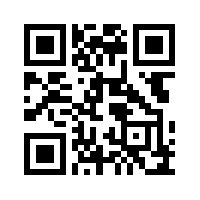
\includegraphics[scale = 0.7]{qrcode_voorbeeld.png}
\caption{Example of simple QR Code.}
\label{qrcode}
\end{figure}
 
 QR Codes can store up to 2,953 [\cite{website:denso-qrcode}] bytes of
 data, which is accessible by scanning the code, with either a laser or a
 digital camera. To scan a QR Code requires a camera that can produce a
 digital image of appropriate quality. This image is then processed by a QR Code library, e.g. the
 well-known ZXing library (see section \ref{sec:zbar}), which decodes the picture and outputs
 the data inside the code. Cellphones are commonly used today because of its portability,
 increasingly powerful hardware and the QR Code technology's simplicity.
 However, an image with a QR Code in can be decoded by any computer with the relevant hardware
 and libraries installed.

\subsection{Zebra Crossing Library}
\label{sec:zbar}

The Zebra Crossing Library (ZXing for short) is a well-known QR Code coding and decoding
library.
It is commonly built into smart phone applications to decode a static image or a video stream,
but a desktop version of the library, called ZBar, is also available and works in a similar
manner. 

To date there has been at least 50 million downloads of the ZXing
bar code scanner app on the Android platform alone, and is currently lies $98^{th}$ in the top
100 of the Google Play Store's most downloaded list [\cite{website:barcodescanner}].

\section{Near Field Communication}

Near Field Communication (NFC) is a relatively new communication standard in the world of
wireless technology. It allows two NFC-enabled devices to wirelessly transmit data to one
another by bringing them to close to one another, typically around 4 t. 

NFC and Radio Frequency Identification (RFID) work on the same principle: when two
devices  (e.g. cellphone, RFID tag, MiFare card, etc.), equipped with an antenna tuned to a
frequency  of 13.56MHz, come into close proximity, they transmit some form of data to one another.

However, there are some important difference between the two technologies. For example, a NFC
system is  an active system, meaning that the device's antenna is always powered and runs off
its own  power supply. NFC devices also have peer-to-peer (p2p) capabilities, meaning that the
two  devices can communicate with one another by both sending and receiving data. RFID systems
on the  other hand, work by having one device act as a listener and the other as a
sender [\cite{website:diff-nfc-rfid}] (e.g. the current SU's student entry control system).

Adding a NFC payment option allows an user with a
NFC-capable smart phone, running on Google's Android operating system (OS), to make their
payments simply  by running an app and swiping their phone across the receiver. Also, due to
the  similarities between NFC and RFID technologies, it may also be possible to add the option
of paying for a product with a SU student or personnel card. However, this needs to be
investigated further before work can start.

\subsection{libnfc}

\subsubsection{nfcpy}

\subsection{Android}

\subsection{Radio Field Identification and Stellenbosch
University Student Cards}

\section{Web Server}

\subsection{Django Web Framework}

\subsection{Elastic Cloud Computing}

\subsection{Apache2}

\section{Encryption}

\subsection{Asymmetric Encryption}

\subsubsection{ElGamal}

\subsubsection{RSA}

\subsection{Base 64}